%!TEX root = main.tex
\chapter{Methods and results}
In this section we will outline what methods we have used for conducting the work.
\section{Data preparation}
\subsection{Data import to database}
We imported the many JSON files to a Postgresql database which allowed us to easily manipulate the data using SQL. We created a single table with the schema shown in Table \ref{table:schema_denormalized}. We decided to compute the time and spatial bins on insertion, thus we only had to compute them once. We created indexes on the following features:start_time, end_time, location, useruuid, spatial_bin, time_bins, country.
Initially we created a normalized database with several relations. We however discovered that a deonormalized database might improve our performance, as we reduce the number of tables and and thus the number of joins required\cite{sanders2001denormalization}. We found This was due to all our interaction with the data only consisting of READs, after the initial insertion of the data. After removing all relations (denormalizing) our performance significantly improved.
\begin{table}[htbp]
\centering

\begin{tabular}{|c|c|c|c|c|c|c|c|c|c|c|}
\hline
\textbf{Field name} & \textbf{Field type}    \\
\hline
id                  & SERIAL PRIMARY KEY     \\
\hline
useruuid            & TEXT NOT NULL          \\
\hline
start\_time         & TIMESTAMPTZ NOT NULL   \\
\hline
end\_time           & TIMESTAMPTZ NOT NULL   \\
\hline
location            & GEOGRAPHY(POINT, 4326) \\
\hline
altitude            & INTEGER NOT NULL       \\
\hline
accuracy            & INTEGER NOT NULL       \\
\hline
region              & TEXT                   \\
\hline
country             & TEXT                   \\
\hline
area                & TEXT                   \\
\hline
place               & TEXT                   \\
\hline
time\_bins          & INTEGER{[}{]} NOT NULL \\
\hline
spatial\_bin        & BIGINT NOT NULL        \\
\hline
\end{tabular}
\caption{Denormalized database schema}
\label{table:schema_denormalized}
\end{table}
\subsection{Data export to Numpy arrays}
We created scripts for exportation to numpy arrays for use in the sklearn module. The users were encoded with K values where K = number of users. The countries were encoded with K values where K = number of countries.

\subsubsection{Binning} \label{ssec:binning}
In the following section the term grid cell or spatial bin will be used synonymously and time interval and time bin aswell.
A spatiotemporal co-occurrence between two users is defined as an instance in which they co-occurred in approximately the same time and approximately the same place.
We have partitioned or binned the globe into a discrete grid where the cells span .001\degree of latitude and longitude on each side (from approximately 43m to 111m\textred{CITE}), and in a discrete time interval of 1-hour.
Thus we say a co-occurrence happens between users $i$ and $j$ if they share the same .001\degree spatial cell C within the same discrete time interval.
 Each grid cell has a unique ID, this is obtained by considering the grid as a matrix and flattening it to a list by traversing from left to right and top to bottom (row-first ordering) and using the list index as an ID. This makes a total possible spatial bin indexes of: $(190\times dec)\times(360\times dec)=68.400.000.000$ with $dec=3$ We calculated the time bins by counting every hour from the start of the day of the earliest date appearing in the dataset, which has the ISO 8601 timestring: "2015-08-09 22:25:33.766+02". The latest day has the ISO 8601 timestring: "2015-12-01 00:59:15.738+01". This leaves us with $2738$ possible time bin IDs. For generating our dataset we count co-occurrences between pairs only once per spatial and time bin.
\begin{figure}[H]
    \hspace*{-1.0cm}
    \centering
    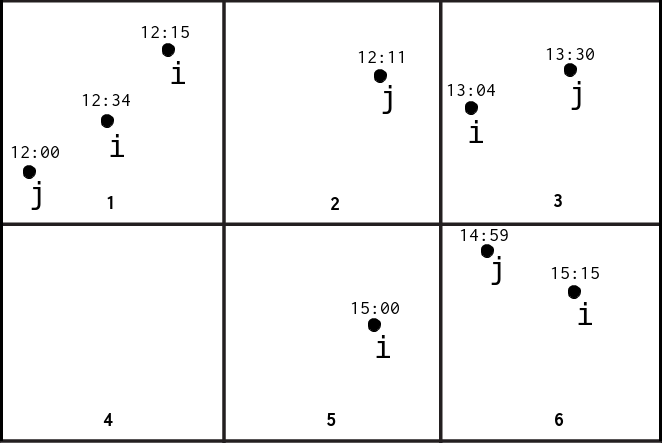
\includegraphics[scale=0.30]{grid}
    \caption{Illustration of spatiotemporal co-occurrences, users $i$ and $j$ have 2 co-occurrences in spatial bin 1 and 3, spatial bin 6 have different time bins.}
    \label{fig:binning}
\end{figure}

\subsection{Visualization}
We used Basemap\cite{basemap}, for plotting all the locations at once and and Leaflet\cite{leaflet} for producing interactive maps to visualize the data, we created a map for visualizing the users location traces over time and we created one that allowed us to see all the co-occurrences that happened between a pair of users. Figure \ref{fig:sweden_locations_hexbin} and \ref{fig:japan_locations_hexbin} shows location updates from Sweden and Japan respectively plotted on a map. We can see location updates happened very often near Sony properties in Lund\cite{sony_headquarters_sweden_lund}, Kista\cite{sony_headquarters_sweden_kista}, and at Ericsson AB in Göteborg\cite{ericsson} for the swedish data, and in Tokyo\cite{sony_headquarters_japan} for the japanese data. Figure \ref{fig:user_pair_at_sony} shows an example of the co-occurrences visualized for a typical pair of users in Sweden having lots of co-occurrences within the Sony perimeter. This enabled us to exclude co-occurrences from these locations from our dataset as we are looking for co-occurrences outside of the users work.
\begin{figure}[H]
    \hspace*{-1.0cm}
    \centering
    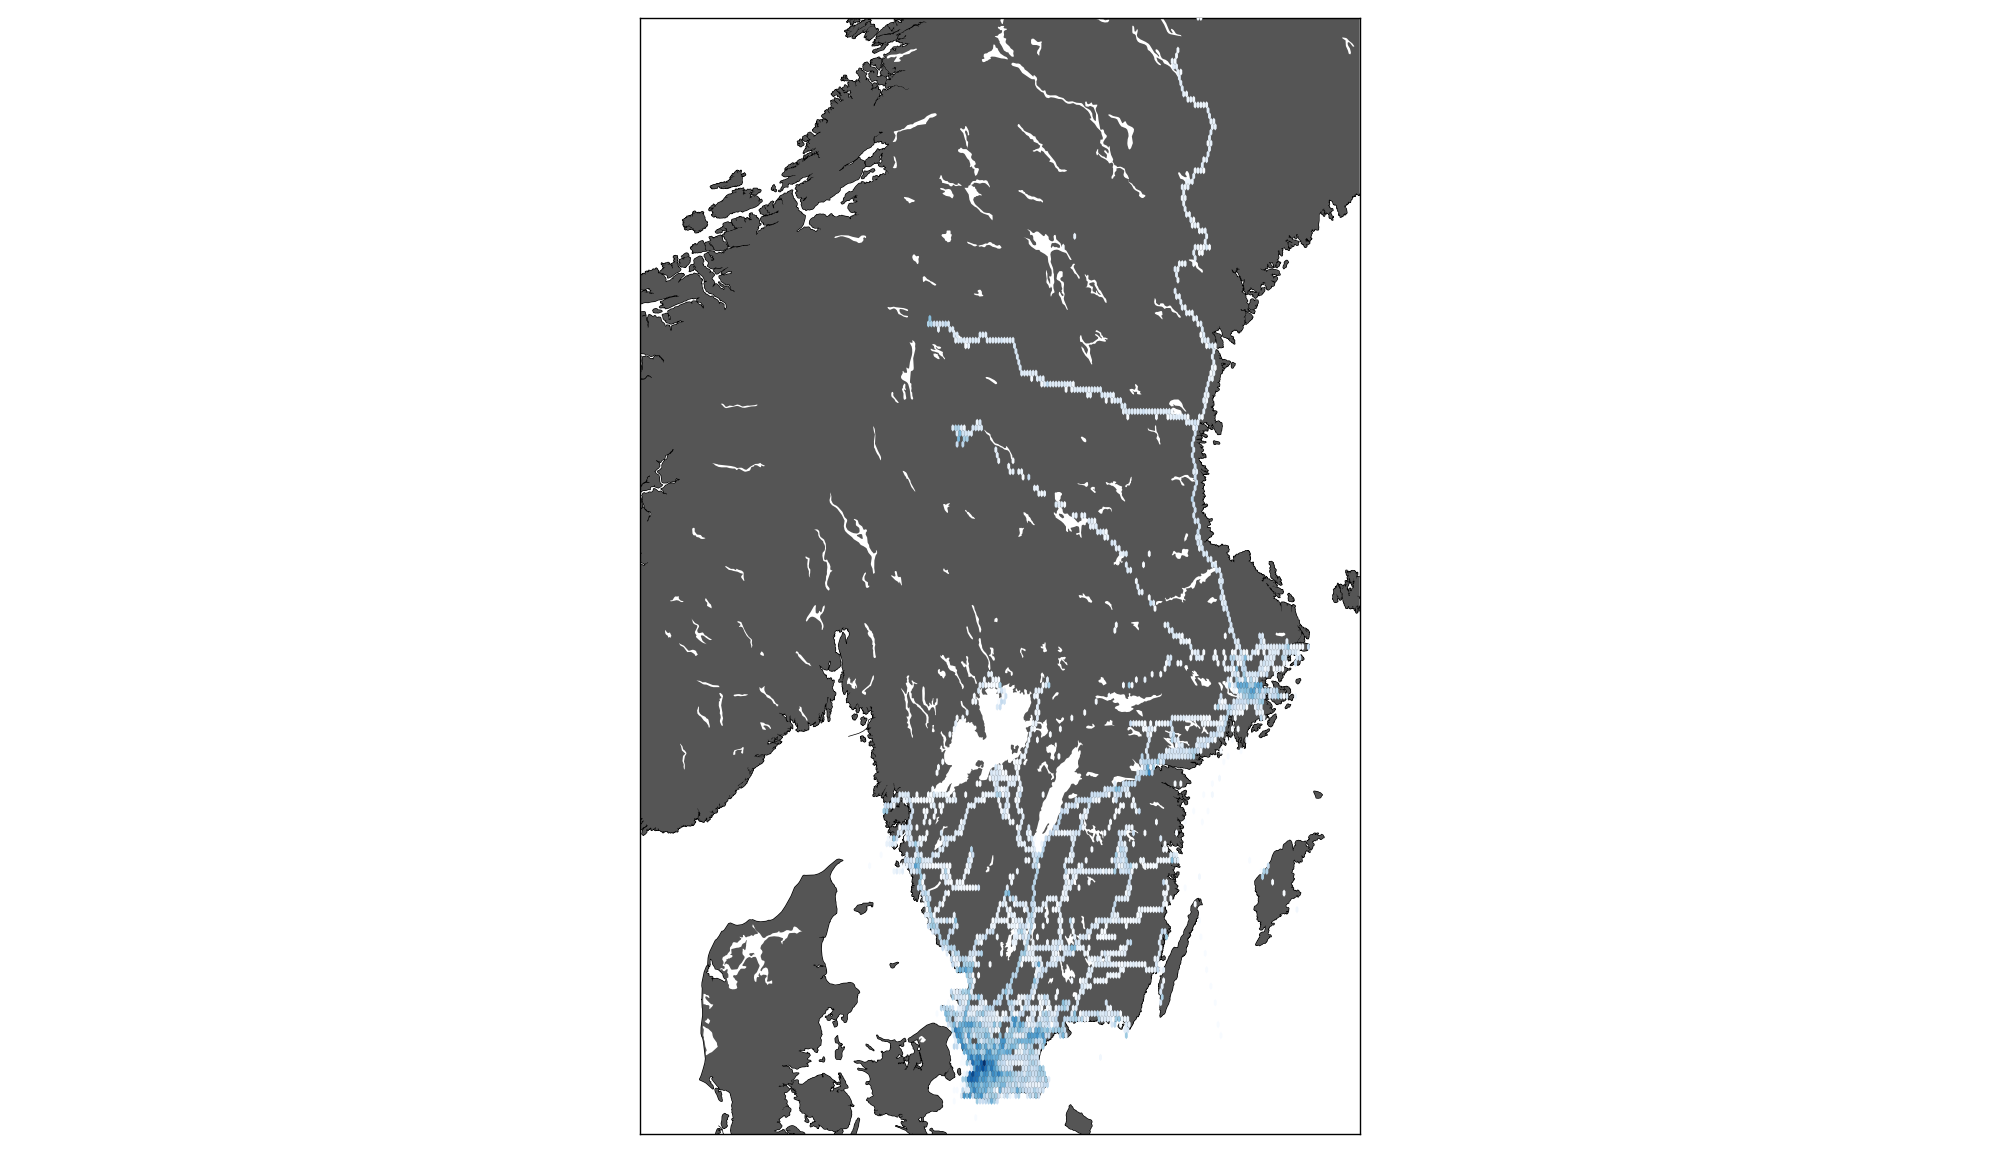
\includegraphics[scale=0.30]{all_locations_sweden}
    \caption{Location updates in Sweden, hexbinned in log scale}
    \label{fig:sweden_locations_hexbin}
\end{figure}
\begin{figure}[H]
    \hspace*{-1.0cm}
    \centering
    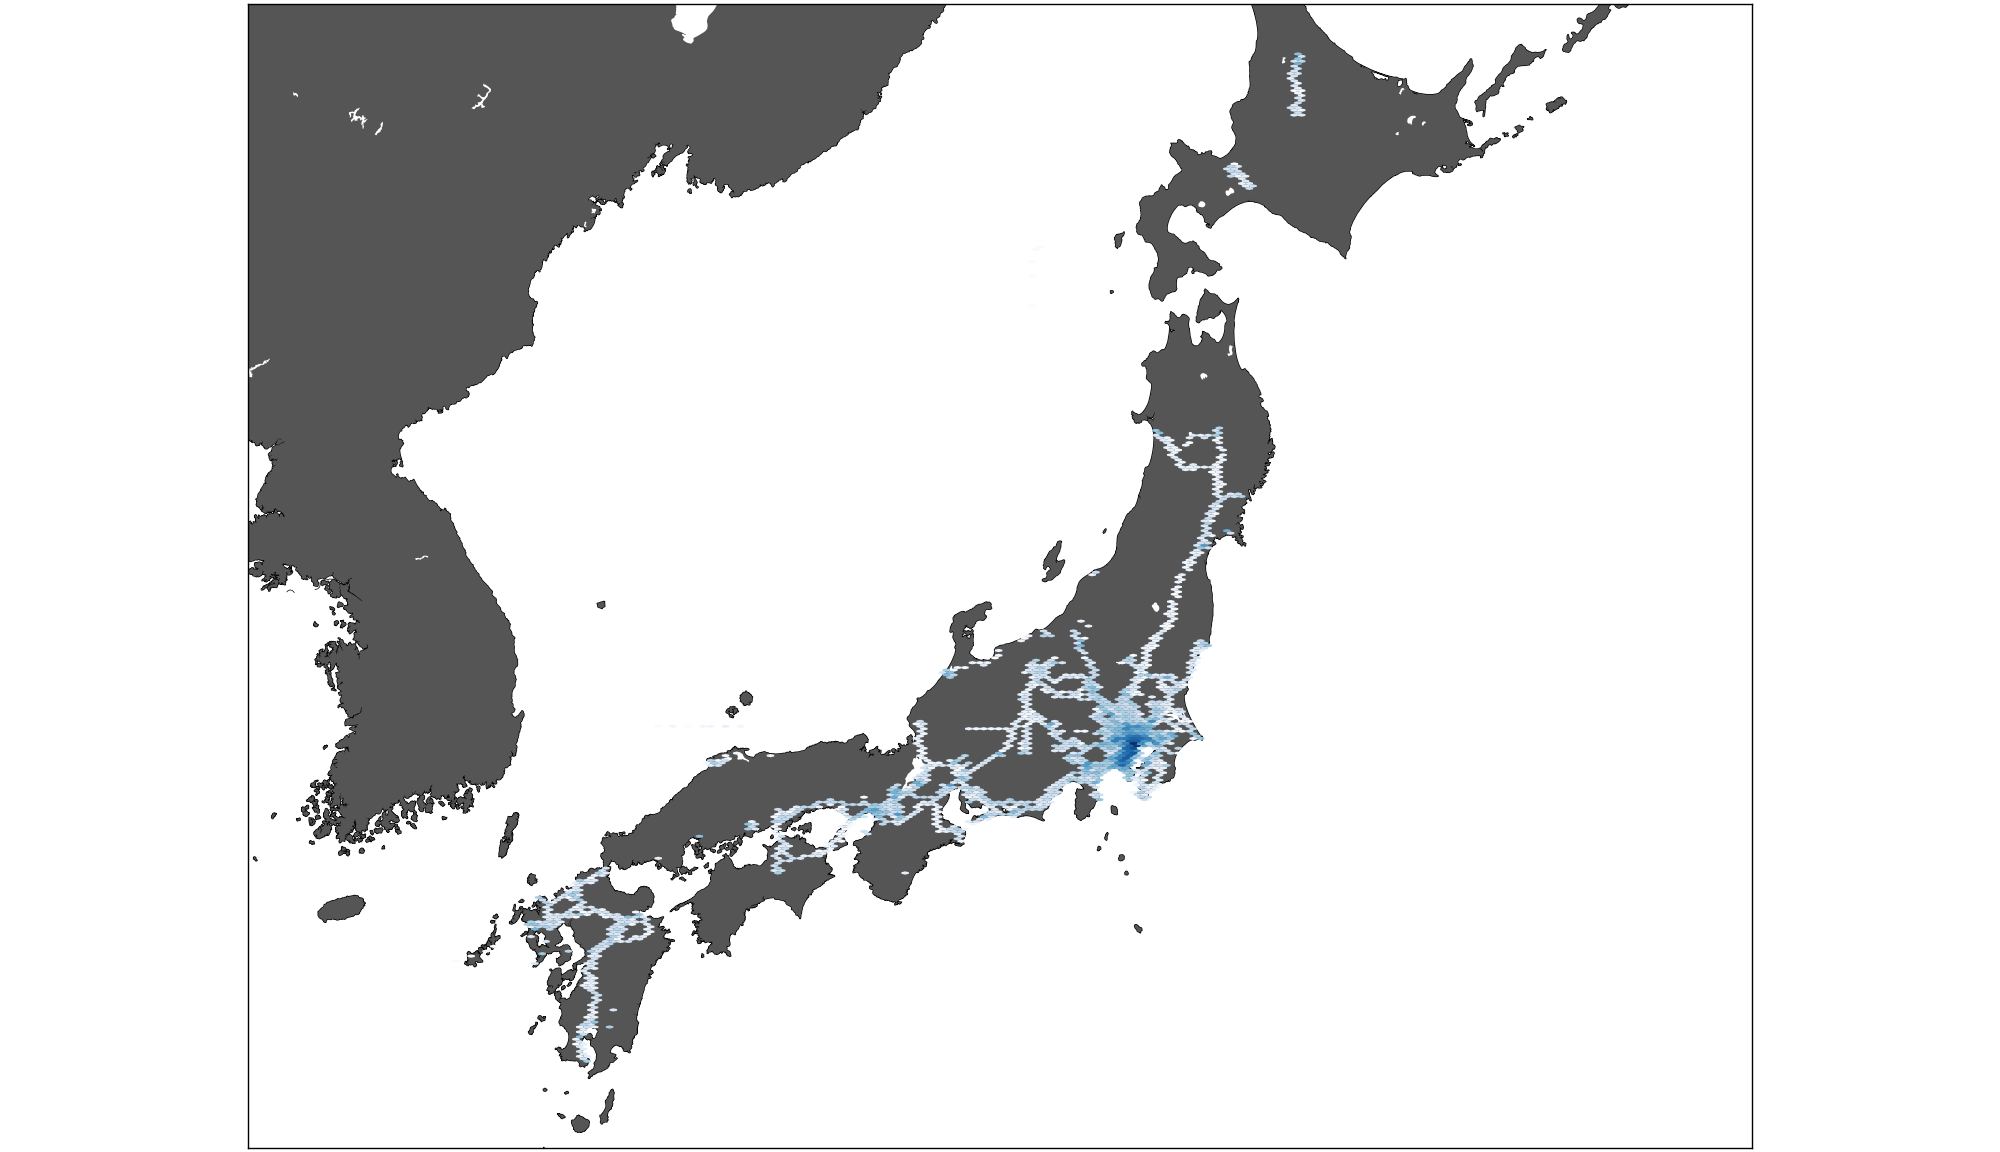
\includegraphics[scale=0.30]{all_locations_japan}
    \caption{Location updates in Japan, hexbinned in log scale}
    \label{fig:japan_locations_hexbin}
\end{figure}
\begin{figure}[H]
    \hspace*{-1.0cm}
    \centering
    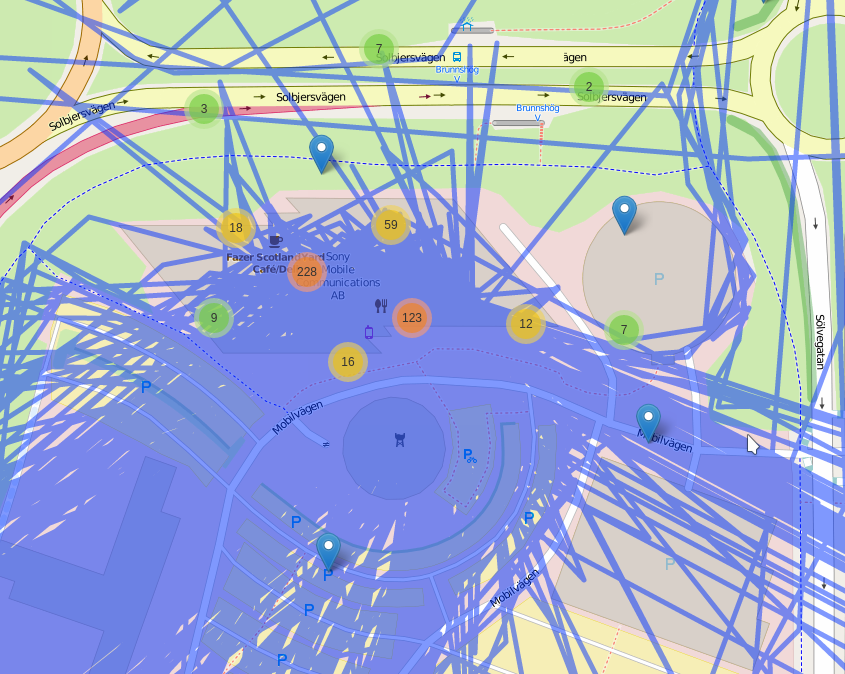
\includegraphics[scale=0.50]{user_pair_at_sony}
    \caption{User pair with high number of co-occurrences for whole period at Sony perimeters}
    \label{fig:user_pair_at_sony}
\end{figure}

We decided to look at just how many location updates and co-occurrences happened inside the Sony perimeter.

\section{Modeling}
In this subsection we will describe the model and features used for prediction.

We will try to answer the following question: Can we predict if people meet in a period based on their spatiotemporal patterns in a previous period.
The models and algorithms we use are implemented in \textit{scikit-learn}\cite{scikit-learn} a Python module for machine learning. 

First we will describe the different features of which our dataset is composed.
\subsection{Features}
\subsubsection{Number of co-occurrences (num\_coocs)}
The total number of co-occurrences between users.
\subsubsection{Diversity of a co-occurrence}
We use the diversity measure taken from the papers of Shahabi and Pham\cite{iRWRfSD}\cite{AEBMtISSfSD}.
Diversity is a measure of how important the spatial locations of the co-occurrences between a pair of persons are, given how many times they appear.
It exists in two forms, one using Shannon entropy another using Rényi entropy, we will use Shannon.
The Shannon entropy is defined by Equation \ref{eq:shannon_entropy}
\begin{equation}
\label{eq:shannon_entropy}
H^S_{ij}=-\sum\limits_{l}P^l_{ij} \log P^l_{ij}= -\sum\limits_{l,c_ij,l\neq 0}\frac{c_{ij,l}}{f_{ij}}\log \frac{c_{ij,l}}{f_{ij}}
\end{equation}
where $f_{ij}$, the \textit{frequency}, is the total number of co-occurrences between user $i$ and user $j$, and $c_{ij,l}$, the \textit{local frequency}, is the total number of co-occurrences between user $i$ and $j$ at location $l$.
From this the diversity is defined by taking the exponential function of the entropy defined in Equation \ref{eq:diversity}:
\begin{equation}
\label{eq:diversity}
D^s_{ij} = exp(H^S_{ij})
\end{equation}

\subsubsection{Weighted frequency}
We use the weighted frequency measure taken from the papers of Shababi and Pham\cite{iRWRfSD}\cite{AEBMtISSfSD}.
Weighted frequency is a measure of how important the co-occurrences at non-popular places are.
The weighed frequency is defined by Equation \ref{eq:weighted_frequency}
\begin{equation}
\label{eq:weighted_frequency}
F_{ij}=\sum\limits_{l}c_{ij,l} \times \exp(-H_l)
\end{equation}
where $H_l$ is the Location Entropy for location \textit{l} defined in Equation \ref{eq:location_entropy}
\begin{equation}
\label{eq:location_entropy}
H_l = \sum\limits_{u, P_{u,l}\neq0} P_{u,l}\log P_{u,l}
\end{equation}
where $P_{u,l}$ is the probability that a location update from location \textit{l} belongs to user \textit{u}.
\subsubsection{Co-occurrences weighted with respect to each location}
We use the weighted co-occurrences measure taken from the master's thesis of P. Sapieżyński\cite{IMM2013-06556}.

\subsubsection{Timely arrival and leaving}
We use the timely arrival and leaving measure taken from the master's thesis of P. Sapieżyński\cite{IMM2013-06556}.

\subsubsection{Unique spatial bins}
The number of unique spatial bins between two users.

\subsubsection{Jaccard index similarity of used apps}
The Jaccard index is a measure used in comparing the similarity of sample sets. We extract what apps two users have used in the period and compute the similarity between them using the Jaccard index.
The Jaccard index is defined in Equation \ref{eq:jaccard_index}
\begin{equation}
\label{eq:jaccard_index}
J(A_i,A_j) = \frac{ |A_i \cap A_j| }{ |A_i \cup A_j | }
\end{equation}
where $A_i$ is the set of apps used by user $i$ and $A_j$ is the set of apps used by user $j$. If $A_i$ and $A_j$ are empty sets we define $J(A_i, A_j) = 1$

\subsection{Results}
Initially we tried to infer friendship based on app usage. We did not have directed call-logs available so we could not reliably say if for example two people were calling each other. However the idea was that if we could find users with a similar timestamp and duration in an app, they could perhaps be communicating with each other either through phone calls or messaging apps. After finding user-pairs that met that criteria we try to validate them looking at their co-occurrences, were they many or few, were they off Sony properties or on, a lot of co-occurrences off sony properties could perhaps indicate a friendship. We identified the Android activity application name and package name for when a user is in a phone call called "Phone" and "package.com.android.incallui" respectively. Furthermore we identified a large number of messaging apps. We tried finding user pairs having activity in the phone app with a start time difference and end time difference of 10 seconds from each other. We looked at co-occurrences between user-pairs found this way and found that they either had a low number of co-occurrences around Sony properties or none at all.

We decided to use a meeting in a next period as a proxy for friendship.

For our training set we found 124 negative samples (did not meet) and 2331 positive samples (did meet), the high number of positive samples is due to the inclusion of location updates in the Sony properties perimeter in our training set. In our test set we found a more moderate 289 negative samples (did not meet) and 191 positive samples (did meet).
First we trained a Logistic Regression classifier which serves as our baseline classifier to compare our other model with. We trained it only with the feature num\_coocs. Next we trained a Random Forest classifier with all of our features.

Due to our imbalanced dataset, the Logistic Regression classifier we trained initially always wanted to just predict the largest prevalent class, positive, in our training dataset.

\subsection{Class Imbalance Problem}
The Class Imbalance Problem is when the total number of samples for one class greatly exceeds the number of samples for a different class. A number of techniques can be used to handle the class imbalance problem, we will use two techniques called oversampling and undersampling\cite{tan2006introduction}. In oversampling you sample the minor sample with replacement until there is an equal number of positive and negative samples. In undersampling you randomly sample from the major class N times where N is the number of minor classes.

\subsection{Performance metrics}
We utilize the precision and recall metrics for evaluating the performance of our models as well as AUC of the ROC Curve.
\subsubsection{Precision}
Precision or the positive predictive value (PPV) is a metric that measures the number of a given class that are correctly identified in proportion to the number of classes that are predicted to be that class.
\subsubsection{Recall}
Recall or the true positive rate (TPR) is a metric that measures the number of a given class that are correctly identified as that class.

In Table \ref{table:models_performance_report} we can see the performance metrics of the different classifiers for the positive (did meet) and negative class (did not meet).

\begin{table}[H]
\centering
\begin{tabular}{|c|c|c|c|c|c|c|c|c|c|c|}
\hline
\textbf{Model} & \textbf{PPV +} & \textbf{TPR +} & \textbf{PPV -} & \textbf{PPV -}   \\
\hline
Logistic Regression (num\_coocs)          & 0.86 & 0.03 & 0.00 & 0.00       \\
\hline
Random Forest (T = 10)    & 0.49 & 0.57 & 0.68 & 0.62\\
\hline
Logistic Regression (num\_coocs, balanced)          & 0.86 & 0.03 & 0.61 & 1.00      \\
\hline
Random Forest (balanced, T = 200)    & 0.44 & 0.79 & 0.71 & 0.34\\
\hline
\end{tabular}
\caption{Models performance metrics}
\label{table:models_performance_report}
\end{table}

We can further look at the number of classes correctly and incorrectly predicted using a Confusion Matrix. Figure \ref{fig:conf_matrix_log_reg} and \ref{fig:conf_matrix_random_forest} shows the confusion matrices for our two models.

\begin{figure}[H]
    \hspace*{-1.0cm}
    \centering
    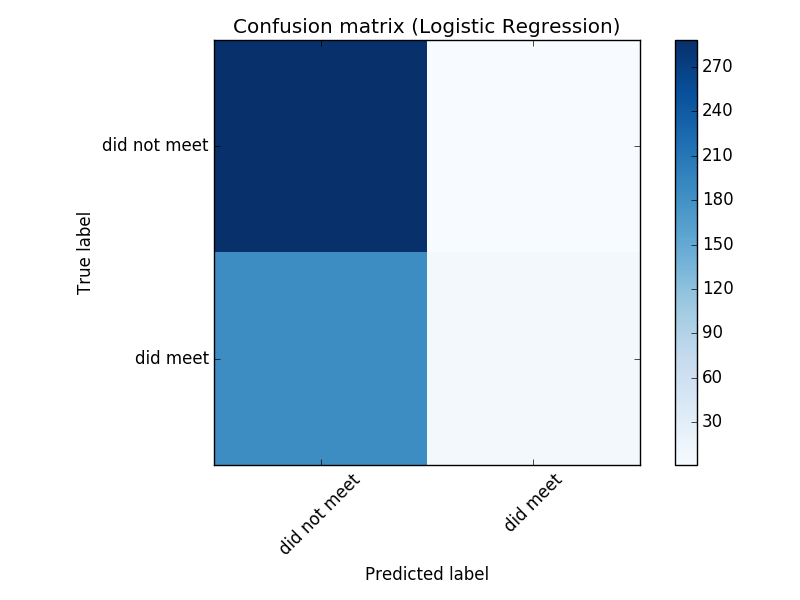
\includegraphics[scale=0.50]{confusion_matrix_log_reg}
    \caption{Confusion matrix for Logistic Regression (num\_coocs feature)}
    \label{fig:conf_matrix_log_reg}
\end{figure}
\begin{figure}[H]
    \hspace*{-1.0cm}
    \centering
    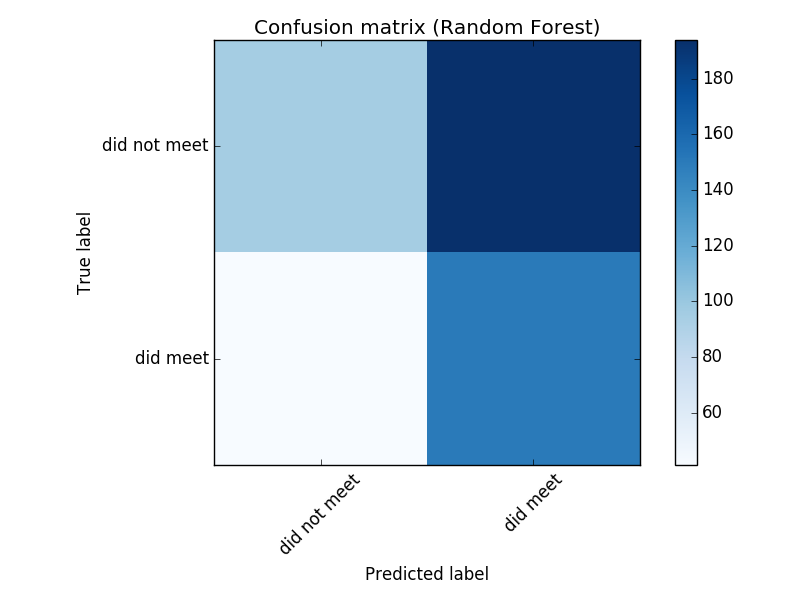
\includegraphics[scale=0.50]{confusion_matrix_random_forest}
    \caption{Confusion matrix for Random Forest (all features, 200 trees)}
    \label{fig:conf_matrix_random_forest}
\end{figure}

Looking at Figure \ref{fig:conf_matrix_log_reg} we see our baseline classifier has a very high 